\section{Valid decorated posets}
\label{sec:valid_decor}

\begin{lemma}
  \label{lem:inhibiting_pair}
  Let $t_1$ and $t_2$ be two transitions in a trace $\theta$ such that $t_1\dashv t_2$. Then $t_2\not\dashv t_1$.
\end{lemma}

\begin{lemma}
  \label{lemma:pos_infl}
  Let $\theta$ a causal trace and let $t_1:M_1\overset{m_1,p_1}{\Rightarrow}N_1$ and $t_2:M_2\overset{m_2,p_2}{\Rightarrow}N_2$ be two transitions in $\theta$. Then the following hold
  \begin{enumerate}
  \item $t_1 <_{\theta} t_2\implies$ there exists a unique cospan $s$ such that $p_1\xrightarrow{+}_s p_2$ and the causal pair of $t_1 <_{\theta} t_2$ is induced by $s$;
  \item $t_1\dashv_{\theta} t_2\implies$ there exists a unique cospan $s$ such that $p_1\xrightarrow{-}_s p_2$ and the inhibiting pair of $t_1\dashv_{\theta} t_2$ is induced by $s$.
  \end{enumerate}
\end{lemma}
\begin{proof}
  \begin{enumerate}
  \item From~\autoref{def:causal_trace} $t_1 <_{\theta} t_2$ implies there exists two transitions $M\overset{m_1,p_1}{\Rightarrow} M_1$ and $M_1\overset{m_2,p_2}{\Rightarrow} M_2$ that are sequential dependent. For any such pair of transitions, using~\autoref{lem:completeness_causal_pair} there exists a causal pair induced by a cospan $s$, which in turns implies that $p_1\xrightarrow{+}_{s}p_2$.

  \item From~\autoref{def:causal_trace} $t_1 \dashv_{\theta} t_2$ implies there exists transitions $M\overset{m_1,p_1}{\Rightarrow} M_1$ inhibiting $M\overset{m_2,p_2}{\Rightarrow} M_2$. For any such pair of transitions, using~\autoref{lem:completeness_inhib_pair} there exists an inhibiting pair induced by a cospan $s$, which in turns implies that $p_1\xrightarrow{-}_s p_2$.
  \end{enumerate}
\end{proof}

\begin{lemma}
  \label{lem:constraint_mj}
  Let $\theta$ a causal trace and let $t_1:M_1\overset{m_1,p_1}{\Rightarrow}N_1$, $t_2:M_2\overset{m_2,p_2}{\Rightarrow}N_2$ and $t_3:M_3\overset{m_3,p_3}{\Rightarrow}N_3$ be three transitions in $\theta$. Let $p_i = L_i\remb K_i \lemb R_i$ be the three rules, for $i\in\{1,2,3\}$.
  \begin{enumerate}
  \item
    \label{lem:constraint_meet}
    If $t_1<_{\theta} t_3$ and $t_2<_{\theta} t_3$, then let $O_1$, $O_2$ be two graphs such that the causal pairs of $t_1<_{\theta} t_3$ and $t_2<_{\theta} t_3$ are induced by $O_1$ and $O_2$ respectively.
%$p_1\xrightarrow{+}_{O_1}p_3$ and $p_2\xrightarrow{+}_{O_2}p_3$.
Let $O_1\remb O\lemb O_2$ be the pullback of the span $O_1\lemb L_3 \remb O_2$. If $t_1\not\dashv t_2$ and $t_2\not\dashv t_1$ then there exists the morphisms $O\emb K_1$ and $O\emb K_2$ such that the diagram below commutes:
    \[
    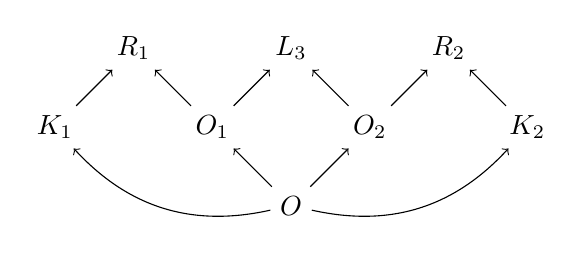
\begin{tikzpicture} %[scale=0.8]
      \node (o) at (0,-1) {\(O\)};
      \node (r3) at (0,1) {\(L_3\)};
      \node (o1) at (-1,0) {\(O_1\)};
      \node (o2) at (1,0) {\(O_2\)};
      \node (r1) at (-2,1) {\(R_1\)};
      \node (r2) at (2,1) {\(R_2\)};
      \node (k1) at (-3,0) {\(K_1\)};
      \node (k2) at (3,0) {\(K_2\)};
      \draw [->] (o) -- (o1);
      \draw [->] (o) -- (o2);
      \draw [->] (o1) -- (r3);
      \draw [->] (o2) -- (r3);
      \draw [->] (o1) -- (r1);
      \draw [->] (o2) -- (r2);
      \draw [->] (k1) -- (r1);
      \draw [->] (k2) -- (r2);
      \draw [->] (o) to [bend left] (k1);
      \draw [->] (o) to [bend right] (k2);
    \end{tikzpicture}
    \]
    Moreover
    \begin{align*}
      t_1^{-1}\dashv t_2^{-1}\implies\text{ there exists the morphisms }O\emb K_1\text{ and }\\
      t_2^{-1}\dashv t_1^{-1}\implies\text{ there exists the morphisms }O\emb K_2.
    \end{align*}
  \item
    \label{lem:constraint_join}
    If $t_3 <_{\theta} t_1$ and $t_3<_{\theta} t_2$, then let $O_1$, $O_2$ be two graphs such that the causal pairs of $t_3 <_{\theta} t_1$ and $t_3<_{\theta} t_2$ are induced by $O_1$ and $O_2$ respectively.
Let $O_1\remb O\lemb O_2$ be the pullback of the span $O_1\lemb R_3 \remb O_2$. If $t_1\not\dashv t_2$ and $t_2\not\dashv t_1$
then there exists the morphisms $O\emb K_1$ and $O\emb K_2$ such that the diagram below commutes:
    \[
    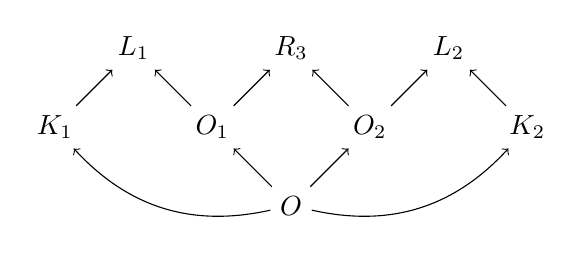
\begin{tikzpicture} %[scale=0.8]
      \node (o) at (0,-1) {\(O\)};
      \node (r3) at (0,1) {\(R_3\)};
      \node (o1) at (-1,0) {\(O_1\)};
      \node (o2) at (1,0) {\(O_2\)};
      \node (r1) at (-2,1) {\(L_1\)};
      \node (r2) at (2,1) {\(L_2\)};
      \node (k1) at (-3,0) {\(K_1\)};
      \node (k2) at (3,0) {\(K_2\)};
      \draw [->] (o) -- (o1);
      \draw [->] (o) -- (o2);
      \draw [->] (o1) -- (r3);
      \draw [->] (o2) -- (r3);
      \draw [->] (o1) -- (r1);
      \draw [->] (o2) -- (r2);
      \draw [->] (k1) -- (r1);
      \draw [->] (k2) -- (r2);
      \draw [->] (o) to [bend left] (k1);
      \draw [->] (o) to [bend right] (k2);
    \end{tikzpicture}
    \]
    Moreover
    \begin{align*}
      t_1\dashv t_2\implies\text{ there exists the morphisms }O\emb K_1\text{ and }\\
      t_2\dashv t_1\implies\text{ there exists the morphisms }O\emb K_2.
    \end{align*}
  \end{enumerate}
\end{lemma}
\begin{proof}
  \begin{enumerate}
  \item
    %% If $\theta$ is a causal trace then we can show that there exists $t_1'$ and $t_2'$ such that $t_1\congr t_1'$, $t_2\congr t_2'$ and such that the transitions $t_1';t_2';t_3$ are composable and such that $t_1'\Diamond_{\text{seq}} t_2'$.
    %% %
    %% Let $\theta'$ be the smallest subtrace of $\theta$ that contains all three transitions $t_1$, $t_2$ and $t_3$. Suppose that $t_1$ occurs before $t_2$, that is $\theta':t_1;\cdots t_2\cdots t_3$.
    %% From $t_2<_{\theta} t_3$ we have that there exists $t_2'$ such that $t_2'< t_3$. It implies that there exists a trace $\theta_1\congr\theta'$ such that $t_2';t_3$ is at the end of $\theta'$.
    %% Using a similar argument as above, there exist $t_1'$ such that $t_1'<_{\theta} t_3$ and we can rewrite $\theta$ to $\theta_1$ ending in $t_1';t_2';t_3$ and with $t_1'\Diamond_{\text{seq}} t_2'$.
    %% %
    %% Consider now the trace $t_1';t_2';t_3$ with $t_2':M_2\remb D_2 \lemb M_3$. We can rewrite $t_1';t_2';t_3$ as $t_2'';t_1'';t_3$, with $t_1'\congr t_1''$ and $t_2'\congr t_2''$. Then we also have the trace $t_2';t_1''^{-1}$ with the two transition sequential independent. Therefore we have that there exists a morphism $R_1\emb D_2$ that makes the diagram commute.

    From $t_1<_{\theta} t_3$ we have that there exists $t_1'\simeq t_1$ such that $t_1';t_3$. Let us denote
$t_1':M_1\remb D_1 \lemb M_3$ the transition $t_1'$. Similarly, from $t_2<_{\theta} t_3$ there exists $t_2\simeq t_2$, $t_2';t_3$ and $t_2':M_2\remb D_2 \lemb M_3$.
    We can show that there exists a morphism $R_1\to D_2$ such that the diagram below commutes iff there is also a morphism $O\to K_2$ that commutes.
    \[
    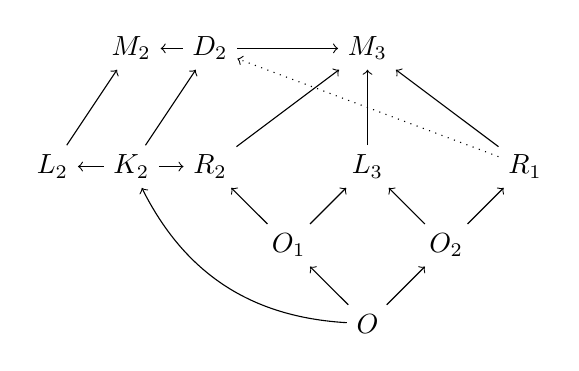
\begin{tikzpicture} %[scale=0.8]
      \node (o) at (0,-1) {\(O\)};
      \node (r3) at (0,1) {\(L_3\)};
      \node (o1) at (-1,0) {\(O_1\)};
      \node (o2) at (1,0) {\(O_2\)};
      \node (r1) at (-2,1) {\(R_2\)};
      \node (r2) at (2,1) {\(R_1\)};
      \node (k1) at (-3,1) {\(K_2\)};
      \node (l1) at (-4,1) {\(L_2\)};
      \node (m3) at (0,2.5) {\(M_3\)};
      \node (d2) at (-2,2.5) {\(D_2\)};
      \node (m2) at (-3,2.5) {\(M_2\)};
      \draw [->] (o) -- (o1);
      \draw [->] (o) -- (o2);
      \draw [->] (o1) -- (r3);
      \draw [->] (o2) -- (r3);
      \draw [->] (o1) -- (r1);
      \draw [->] (o2) -- (r2);
      \draw [->] (k1) -- (r1);
      \draw [->] (o) to [bend left] (k1);
      \draw [->] (k1) -- (l1);
      \draw [->] (d2) -- (m2);
      \draw [->] (d2) -- (m3);
      \draw [->] (k1) -- (d2);
      \draw [->] (l1) -- (m2);
      \draw [->] (r1) -- (m3);
      \draw [->] (r3) -- (m3);
      \draw [->] (r2) -- (m3);
      \draw [dotted,->] (r2) -- (d2);
    \end{tikzpicture}
    \]
    We have then that if $t_2\not\dashv t_1$ then the morphism $O\to K_2$ above exists and moreover if there is no morphism $O\to K_2$ that commutes then $t_2\dashv t_1$. We reason similarly for $t_1\dashv t_2$.

    From~\autoref{lem:inhibiting_pair}, if $t_2\dashv t_1$ then $t_1\not\dashv t_2$ and hence there exists $O\to K_1$ that commutes.
    \item The proof is similar to the one above.
  \end{enumerate}
\end{proof}

Inutuitively,~\autoref{lem:constraint_mj} says that if two events cannot \emph{produce} the same resource (\autoref{lem:constraint_meet}) and the same resource cannot be \emph{consumed} twice (\autoref{lem:constraint_join}). Let us give some examples.
\begin{example}
  For the following rules:
  \[
  r_1:\varepsilon \Rightarrow A,B \qquad r_2: \varepsilon \Rightarrow A,C \qquad r_3: A,B,C \Rightarrow D
  \]
  there is a trace where $t_1<t_3$ and $t_2<t_3$, however both cannot produce $A$:
    \[
    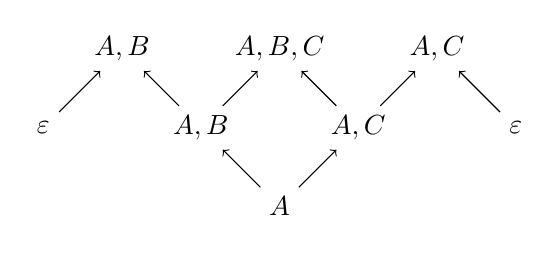
\begin{tikzpicture} %[scale=0.8]
      \node (o) at (0,-1) {\(A\)};
      \node (r3) at (0,1) {\(A,B,C\)};
      \node (o1) at (-1,0) {\(A,B\)};
      \node (o2) at (1,0) {\(A,C\)};
      \node (r1) at (-2,1) {\(A,B\)};
      \node (r2) at (2,1) {\(A,C\)};
      \node (k1) at (-3,0) {\(\varepsilon\)};
      \node (k2) at (3,0) {\(\varepsilon\)};
      \draw [->] (o) -- (o1);
      \draw [->] (o) -- (o2);
      \draw [->] (o1) -- (r3);
      \draw [->] (o2) -- (r3);
      \draw [->] (o1) -- (r1);
      \draw [->] (o2) -- (r2);
      \draw [->] (k1) -- (r1);
      \draw [->] (k2) -- (r2);
    \end{tikzpicture}
    \]
  %% \[
  %% t_1: A \Rightarrow A,B \qquad t_2: A \Rightarrow A,C \qquad t_3: A,B,C \Rightarrow D
  %% \]
  %% we can indeed have that both $t_1<t_3$ and $t_2<t_3$.
\end{example}
\begin{example}
  Consider the transitions
  \[
  t_3: \varepsilon \Rightarrow A\qquad t_1: A\Rightarrow \varepsilon \qquad t_2: A\Rightarrow \varepsilon
  \]
  for which there is no trace where both $t_3<t_1$ and $t_3<t_2$ hold. The resource $A$ produced by $t_1$ can only be consumed once.
  If, however, $t_1$ and $t_2$ do not consume $A$ but preserve it:
  \[
  t_3: \varepsilon \Rightarrow A\qquad t_1: A\Rightarrow A,B \qquad t_2: A\Rightarrow A,C
  \]
  then indeed both $t_1<t_3$ and $t_2<t_3$ hold.
\end{example}
  %% Note that though the following trace $\theta$, produced by transitions $t_3;t_1;t_2$, is valid
  %% \[
  %% \theta:\varepsilon \Rightarrow A \Rightarrow A, B\Rightarrow B\qquad t_3: \varepsilon \Rightarrow A\qquad t_1: A\Rightarrow A,B\qquad t_2: A\Rightarrow \varepsilon
  %% \]
  %% we cannot deduce $t_3<t_2'$, for $t_2'\congr t_2$, as in the trace $\theta$ above, transitions cannot commute.
\begin{example}
  For a trace $t_1;t_2;t_3$ with the transitions
  \[
  t_1: A \Rightarrow A,B\qquad t_2: A,B\Rightarrow B,C \qquad t_3: B,C\Rightarrow D
  \]
  one cannot deduce $t_1<t_3$, as transitions $t_1$ and $t_2$ do not commute.
\end{example}


\begin{lemma}
  \label{lem:constraint_inhibit}
  Let $\theta$ a causal trace and let $t_1:M_1\overset{m_1,p_1}{\Rightarrow}N_1$ and $t_2:M_2\overset{m_2,p_2}{\Rightarrow}N_2$ be two transitions in $\theta$.
  If $t_1 \leq t_2$ then $t_2\not\dashv t_1$.
\end{lemma}
\begin{proof}[Proof sketch]
  One cannot commute $t_1$ and $t_2$ such that $t_1':M\overset{m_1,p_1}{\Rightarrow}N_1$ and $t_2':M\overset{m_2,p_2}{\Rightarrow}N_2$, for some $t_1'\simeq t_1$, $t_2'\simeq t_2$. Therefore one cannot deduce that the pair are not parallel independent.
\end{proof}


\begin{mdframed}[backgroundcolor=blue!20]
to do: define alpha  on decorated posets.
\end{mdframed}

\begin{lemma}
  \label{prop:constraints_poset}
  For any causal trace $\theta$, $\alpha(\theta)$ is a valid decorated poset.
\end{lemma}
\begin{proof}
  It is straigthforward from~\autoref{def:causal_trace},~\autoref{lem:inhibiting_pair},~\autoref{lem:constraint_inhibit} and \autoref{lem:constraint_mj}.
\end{proof}
